%!TEX root = FHI-aims.tex
\section{Many-Body Dispersion (MBD) energy}

The non-local many-body dispersion (MBD) or correlation energy 
(with forces and stress) is computed using a system of coupled atomic response
functions~\cite{MBD,QHORPA}.

In fact, the code includes three separate implementations of the MBD
approach. The text below first describes the approach with the
broadest applicability (including efficient implementations of total
energy gradients). The two other implementations are described in a
separate section.
 
\begin{figure}[h]
\begin{center}
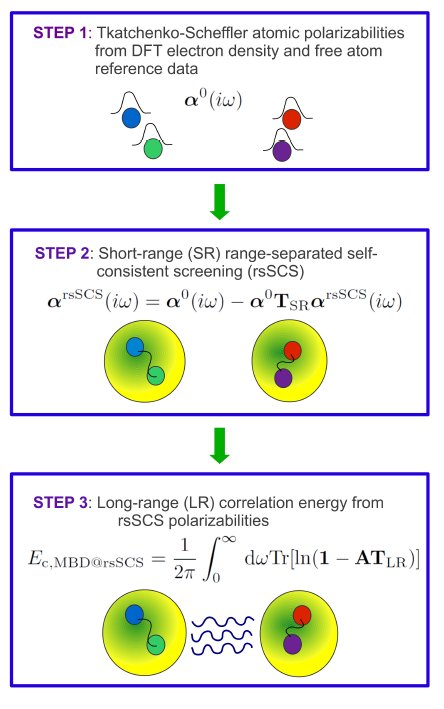
\includegraphics[scale=0.6,trim=0cm 0cm 0cm 0cm]{MBD.jpg}
\end{center}
\caption{Schematic description of the MBD@rsSCS method.} 
\label{mbdmethodfigure}
\end{figure}
The MBD method implemented in FHI-aims is the so-called range-separated
MBD@rsSCS method~\cite{MBD,QHORPA}. 
The dynamic polarizability $\alpha(i\omega)$ as a function of imaginary 
frequency for a molecule or extended system is obtained as a solution to the 
self-consistent screening equation using a regularized dipole potential. The 
standard output of FHI-aims contains the upper triangular part of the dynamic 
polarizability tensor: 
\begin{verbatim}
| Many-Body Dispersion (MBD@rsSCS) energy
| Dynamic polarizability of unit cell alpha(iw)(bohr^3)
|---------------------------------------------------------------------------
| omega(Ha)   XX         YY         ZZ         YZ         XZ         XY
| 0.000000  0.717E+04  0.724E+04  0.609E+04  0.180E+01  0.752E+01  0.224E+00
| 0.039290  0.704E+04  0.711E+04  0.599E+04  0.175E+01  0.762E+01  0.222E+00
| 0.118358  0.616E+04  0.623E+04  0.529E+04  0.141E+01  0.816E+01  0.201E+00
\end{verbatim}
Furthermore, the atom projected static polarizability $\alpha(0)$ and vdW 
$C_{6}$ coefficient for each atom in a system are given as follows:
\begin{verbatim}
|---------------------------------------------------------------------------
| Partitioned C6 (hartree bohr^6) | alpha(bohr^3)  of atom in unit cell
|---------------------------------------------------------------------------
| ATOM   1  Zn  189.850551         30.849981
| ATOM   2  Zn  194.746383         31.378482
| ATOM   3  O   10.645313          2.411834
| ATOM   4  O   10.522485          2.335995
\end{verbatim}
Please note that the above values are derived using a range-separated dipole 
potential. For more technical details see Refs.~\cite{MBD,QHORPA}.

Analytical forces and stress are implemented for MBD@rsSCS, with the 
following caveat.
The total nuclear derivatives of the MBD energy consist of the direct terms,
and the implicit terms arising from the dependence on the Hirshfeld volumes,
which in turn depend on nuclear positions.
Currently, the latter implicit terms are neglected (work in progress),
however, preliminary testing suggests that these terms are negligible
in many systems.
In fact, the error arising from neglecting these terms seems to be in 
general comparable to or smaller than the inherent numerical noise in 
the Kohn--Sham forces.
Having said that, please report any observed discrepancies in the forces 
during geometry relaxations or MD simulations to 
\href{mailto:jhermann@fhi-berlin.mpg.de?subject=\%5Baims\%20mbd-std\%5D}{jhermann@fhi-berlin.mpg.de}.

\subsection*{Tags for general section of \texttt{control.in}:}

The most capable implementation of MBD in FHI-aims is provided by the
\href{https://github.com/azag0/libmbd}{Libmbd} library. Libmbd provides a fully distributed and
parallelized implementation of the MBD energy, forces, and stress tensor.

The \texttt{control.in} tag for the Libmbd implementation follows the same structure as the default implementation, with some differences in the available options.

\keydefinition{many\_body\_dispersion}{control.in}{
  \noindent
  Usage: \keyword{many\_body\_dispersion} \texttt{[option=value\ldots]}\\
}

\begin{itemize}
  \item \option{k\_grid=<nk1>:<nk2>:<nk3>} [default: taken from
    \texttt{k\_grid}] specifies the $k$-point grid used for sampling
  the first Brillouin zone in the MBD calculation. The grid is shifted
  by half a distance between the $k$-points from the
  $\Gamma$-point. [only for periodic systems] 
  \item \option{supercell=<n1>:<n2>:<n3>} specifies the supercell size that
  is used in the real-space formulation of MBD\@. This is considered
  inferior to the reciprocal formulation and should be used only for
  testing. Only one of \option{k\_grid} and \option{supercell} can be
  specified. [only for periodic systems]
  \item \option{beta=<real>} [default: depends on XC functional] sets the
  damping parameter $\beta$.
  \item \option{freq\_grid=<integer>} [default: 15] controls the size of
  the imaginary-frequency grid used for the Casimir--Polder integral. 
  [same as \texttt{omega\_grid} \\
  in \keyword{many\_body\_dispersion\_pre2019}]
  \item \option{zero\_negative=<logical>} [default: .false.] controls whether negative eigenvalues of the MBD Hamiltonian are zeroed out or cause the calculation to abort
\end{itemize}

Examples:
\begin{itemize}
    \item \verb+many_body_dispersion+ (this uses the default settings)
    \item \verb+many_body_dispersion k_grid=3:3:3+ (explicit settings of a $3\times3\times3$ $k$-point grid)
    \item \verb+many_body_dispersion self_consistent=.true. ewald=.false.+ (turns on self-consistency and switches off the Ewald summation)
    \item \verb+many_body_dispersion k_grid=10:1:1+\\
          \verb+many_body_dispersion vacuum=.false.:.true.:.true.+\\
          (multiline, explicit $k$-point grid and vacuum settings)
\end{itemize}


\subsection*{Legacy FHI-aims internal implementation (pre 2019 default)}

\keydefinition{many\_body\_dispersion\_pre2019}{control.in}{
  \noindent
  Usage: \keyword{many\_body\_dispersion\_pre2019} \texttt{[option=value\ldots]}\\[1.0ex]
  Purpose: Calculates the MBD@rsSCS energy for the active XC
  functional (available for PBE, PBE0, and HSE). \\
}
This was the default method prior the official 2019 FHI-aims release. 
The default has changed to the libmbd implementation \keyword{many\_body\_dispersion} 
described above.

Sane defaults are provided, so in principle no further input is
needed. Nevertheless, the following \texttt{option=value} pairs are
available. Note that these can be specified either all on a single line,
or across multiple lines, each starting with \texttt{many\_body\_dispersion}.
 
\begin{itemize}
  \item \option{k\_grid=<nk1>:<nk2>:<nk3>} [default: taken from
    \texttt{k\_grid}] specifies the $k$-point grid used for sampling
  the first Brillouin zone in the MBD calculation. The grid is shifted
  by half a distance between the $k$-points from the
  $\Gamma$-point. [only for periodic systems] 
  \item \option{supercell=<n1>:<n2>:<n3>} specifies the supercell size that
  is used in the real-space formulation of MBD\@. This is considered
  inferior to the reciprocal formulation and should be used only for
  testing. Only one of \option{k\_grid} and \option{supercell} can be
  specified. [only for periodic systems] 
  \item \option{vacuum=<a>:<b>:<c>} [default: all \texttt{.false.}] controls
  whether some of the lattice vectors correspond to vacuum
  dimensions. 
  \item \option{self\_consistent=<logical>} [default: \texttt{.false.}]
  controls the calculation of the MBD XC potential. 
  \item \option{old\_hirshfeld=<logical>} [default: \texttt{.false.}]
  controls whether the older implementation of the Hirshfeld volumes
  is used. Only the new implementation supports self-consistent
  calculations. Note that the Hirshfeld output printed by FHI-aims is
  always generated by the older implementation, irrespective of this
  option. 
  \item \option{beta=<real>} [default: depends on XC functional] sets the
  damping parameter $\beta$. 
  \item \option{omega\_grid=<integer>} [default: 15] controls the size of
  the imaginary-frequency grid used for the Casimir--Polder integral. 
  \item \option{ewald=<logical>} [default: \texttt{.true.}] controls whether
  Ewald summation is used for the dipole tensor in periodic systems. 
  \item \option{max\_negative\_eigvals=<integer>} [default: 3]
  controls how many negative eigenvalues can be ignored (by setting them to zero).
\end{itemize}

\subsection*{Alternative implementation of the MBD method}

An independent, alternative implementation of the MBD method is also
available (useful for testing). This version lacks analytical forces
and the reciprocal-space formulation for periodic systems, but uses
scaLAPACK, which can be potentially useful for massive cluster
calculations (thousands of atoms). 

\keydefinition{many\_body\_dispersion\_alt}{control.in}
{
  \noindent
  Usage: \keyword{many\_body\_dispersion\_alt} \\[1.0ex]
  Purpose: Calculates the MBD@rsSCS energy for a given xc functional
  (available for PBE, PBE0, and HSE functionals). 
\\
}

\keydefinition{mbd\_scs\_vacuum\_axis}{control.in}
{
  \noindent
  Usage: \keyword{mbd\_scs\_vacuum\_axis} \option{flag flag flag} \\[1.0ex]
  Purpose: This keyword specifies direction of the vacuum region in case of a low-dimensional system.\\
  Default: No vacuum \keyword{mbd\_scs\_vacuum\_axis} \texttt{.false.  .false.  .false.} \\
  For example, in the case of {\it periodic} slab along $xy$ directions the keyword\\
  \keyword{mbd\_scs\_vacuum\_axis} \texttt{.false.  .false.  .true.} is needed to specify  
  $z$ as vacuum direction in MBD/SCS calculation.
}

\keydefinition{mbd\_cfdm\_dip\_cutoff}{control.in}
{
  \noindent
  Usage: \keyword{mbd\_cfdm\_dip\_cutoff} \option{value} \\[1.0ex]
  Purpose: Radius used to integrate the dipole field in a {\it periodic} MBD calculation (internal default value =100.0 Angstrom)
}

\keydefinition{mbd\_scs\_dip\_cutoff}{control.in}
{
  \noindent
  Usage: \keyword{mbd\_scs\_dip\_cutoff} \option{value} \\[1.0ex]
  Purpose: Radius used to integrate the dipole field in a {\it periodic} SCS calculation (internal default value =120.0 Angstrom) 
}
\keydefinition{mbd\_supercell\_cutoff}{control.in}
{
  \noindent
  Usage: \keyword{mbd\_supercell\_cutoff} \option{value} \\[1.0ex]
  Purpose: Radius used to construct the supercell in {\it periodic} MBD@rsSCS calculations. (internal default value = 25 Angstrom)
  NOTE: The convergence with respect to the value of \keyword{mbd\_supercell\_cutoff} must be carefully tested for periodic systems with low symmetry.
}

\keydefinition{mbd\_eigensolver}{control.in}
{
  \noindent 
  Usage: \keyword{mbd\_eigensolver} \option{type} \\[1.0ex]
  Purpose: Algorithm used to solve the MBD eigenvalue problem.\\[1.0ex]
  \option{type} is a keyword (string) which specifies the eigenvalue solver
    used. Default: \texttt{lapack} for serial or mpi runs without scaLAPACK  
    support. \texttt{scalapack} for mpi runs with available scaLAPACK library. \\ 
}
Available options for the eigensolver, \option{type}, are:
\begin{itemize}
  \item \texttt{lapack} : \textbf{Preferred 
    serial eigensolver implementation}. Lapack-based, and similar to the
    divide\&conquer based standard solver provided by Lapack.
  \item \texttt{scalapack} :  Fully memory-parallel implementation of 
    the eigenvalue solver based on scaLAPACK.
  \item \texttt{elpa} : \textbf{Preferred 
    parallel eigensolver implementation. Uses the ELPA eigensolver library.}
    Same functionality as \texttt{scalapack}, however, substantially 
    rewritten for an overall speedup and much improved scalability.
    Recommended on shared-memory platforms and distributed systems with any
    decent communication. \\
    Note that you must set the shell variable \texttt{OMP\_NUM\_THREADS}=1 
    prior to running FHI-aims on some platforms. 
    (see Appendix \ref{appendix_trouble_shooting})
\end{itemize}
The scaLAPACK or ELPA eigensolvers are only available if scaLAPACK
support has been compiled into the FHI-aims binary---see the Makefile
for more information. 

In fact, the default parallel eigensolver in FHI-aims is the ``ELPA''
eigensolver, which uses some scalapack infrastructure but has been
rewritten from the ground up for much improved parallel scalability.

On mildly parallel platforms (no more than tens
of CPUs) and for normal system sizes (not significantly larger than
$\sim$100 atoms), it is often acceptable to use the serial
\texttt{lapack} eigensolver instead of the fully parallel
\texttt{elpa} or \texttt{scalapack}.

NOTE: Care must be taken for parallel MBD calculations if \texttt{lapack} is chosen: MBD uses a supercell that is often larger than the specified unit cell. The current implementation allocates a 3{\it N}x3{\it N} matrix on every thread. If there is a memory problem it is worth to compile FHI-aims with scaLAPACK support and choose \texttt{elpa} or \texttt{scalapack}.

%\subsection*{Experimental implementation of the MBD method}
%
%A third, independent implementation of MBD also exists. Since this code is mainly intended for development purposes and prototyping, no support is provided. However, interested users can contact \href{mailto:jhermann@fhi-berlin.mpg.de?subject=\%5Baims\%20mbd-dev\%5D}{jhermann@fhi-berlin.mpg.de} for further information.
%
%\keydefinition{many\_body\_dispersion\_dev}{control.in}
%{
%  \noindent 
%  Usage: \keyword{many\_body\_dispersion\_dev} \texttt{[\ldots]} \\[1.0ex]
%  Purpose: Activates the experimental MBD implementation. 
%}
